In Versuch DT2 ging es um die schaltungstechnische Realisierung eines seriellen, 4-Bit-Rechenwerkes. Es sollen zunächst zwei 4-Bit-Dualzahlen in zwei Schieberegister parallel eingeschrieben werden, welche anschließend seriell mittels eines Vollsubtrahierers subtrahiert werden sollen. Das Ergebnis soll in einem der beiden Schieberegister gespeichert werden. Außerdem ist ein Systemtakt zu erzeugen, damit das Ergebnis nicht nocheinmal verrechnet wird.\par
Dazu sollten zunächst drei einzelne Schaltungen entwickelt werden. Die erste Schaltung dient zur Einlesung der beiden Dualzahlen in die Schieberegister. Mit Hilfe der zweiten Schaltung wird ein Systemtakt erzeugt. Die dritte Schaltung enthält die Elemente der vorherigen beiden und verbindet sie mit einem Vollsubtrahierer. Die Entleihung wird auch gespeichert und bei einem negativen Ergebnis soll eine LED leuchten. Ist das Ergebnis negativ, müsste noch das Zweierkomplement gebildet werden, weshalb das angezeigte Ergebnis nicht korrekt ist.\par
Am Versuchstag sollten die einzelnen Teilschaltungen auf einem Board (siehe Bild) aufgebaut und in ihrer Funktion vorgeführt werden. Es traten keine Probleme auf und der Subtrahierer funktionierte auf Anhieb einwandfrei.\par
Die vorbereitenden Aufgaben konnten ebenfalls ohne größere Probleme in der vorgegebenen Zeit gelöst werden.


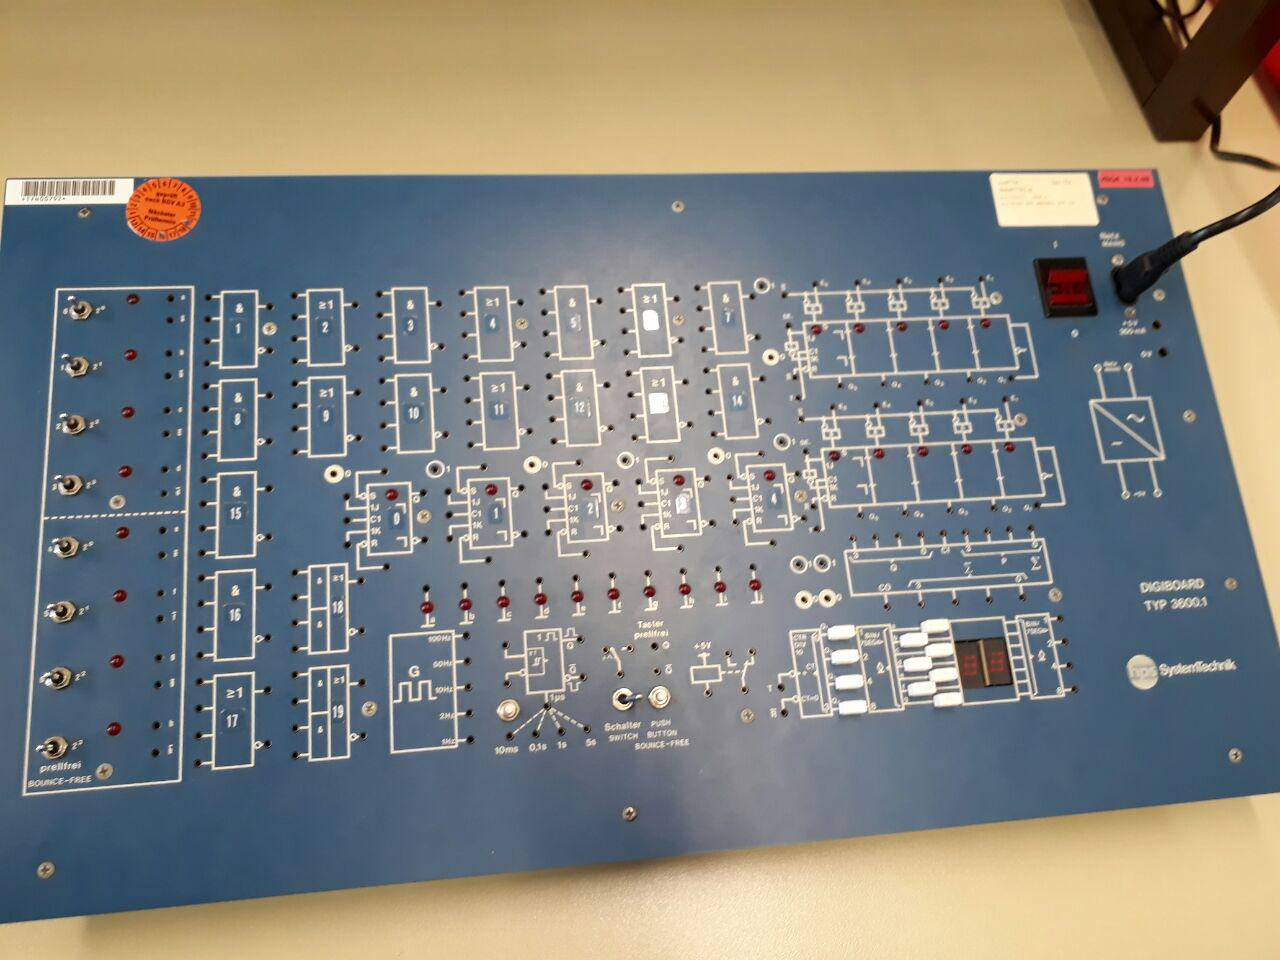
\includegraphics[width=0.75\columnwidth]{DT2Graphics/Board.jpg}
